\documentclass[11pt]{article}    	
\usepackage{geometry}      
\usepackage[latin1]{inputenc}  
\usepackage[T1]{fontenc}          		
\geometry{a4paper} 
\usepackage{scrextend}  
\usepackage{tikz}
\usepackage{framed}
\usepackage{graphicx}
\usepackage{fancyhdr}

\pagestyle{fancy}
\rhead{Iacopo Sprenger 284074}
\lhead{Programmation I}
\setlength{\headheight}{14pt}
					
					
\begin{document}
\begin{center}
\Large \textbf{Projet d'Automne: Me too ?}
\end{center}
Une fois les param�tres entrez par l'utilisateur v�rifi�s, le programme commence les simulations. Le tout est structur� en trois boucles tout a l'ext�rieur il y a la boucle des contextes ensuite la boucle du taux de vaccination et finalement une boucle pour le nombre de simulations. 
\begin{figure}[htb]
\begin{framed}
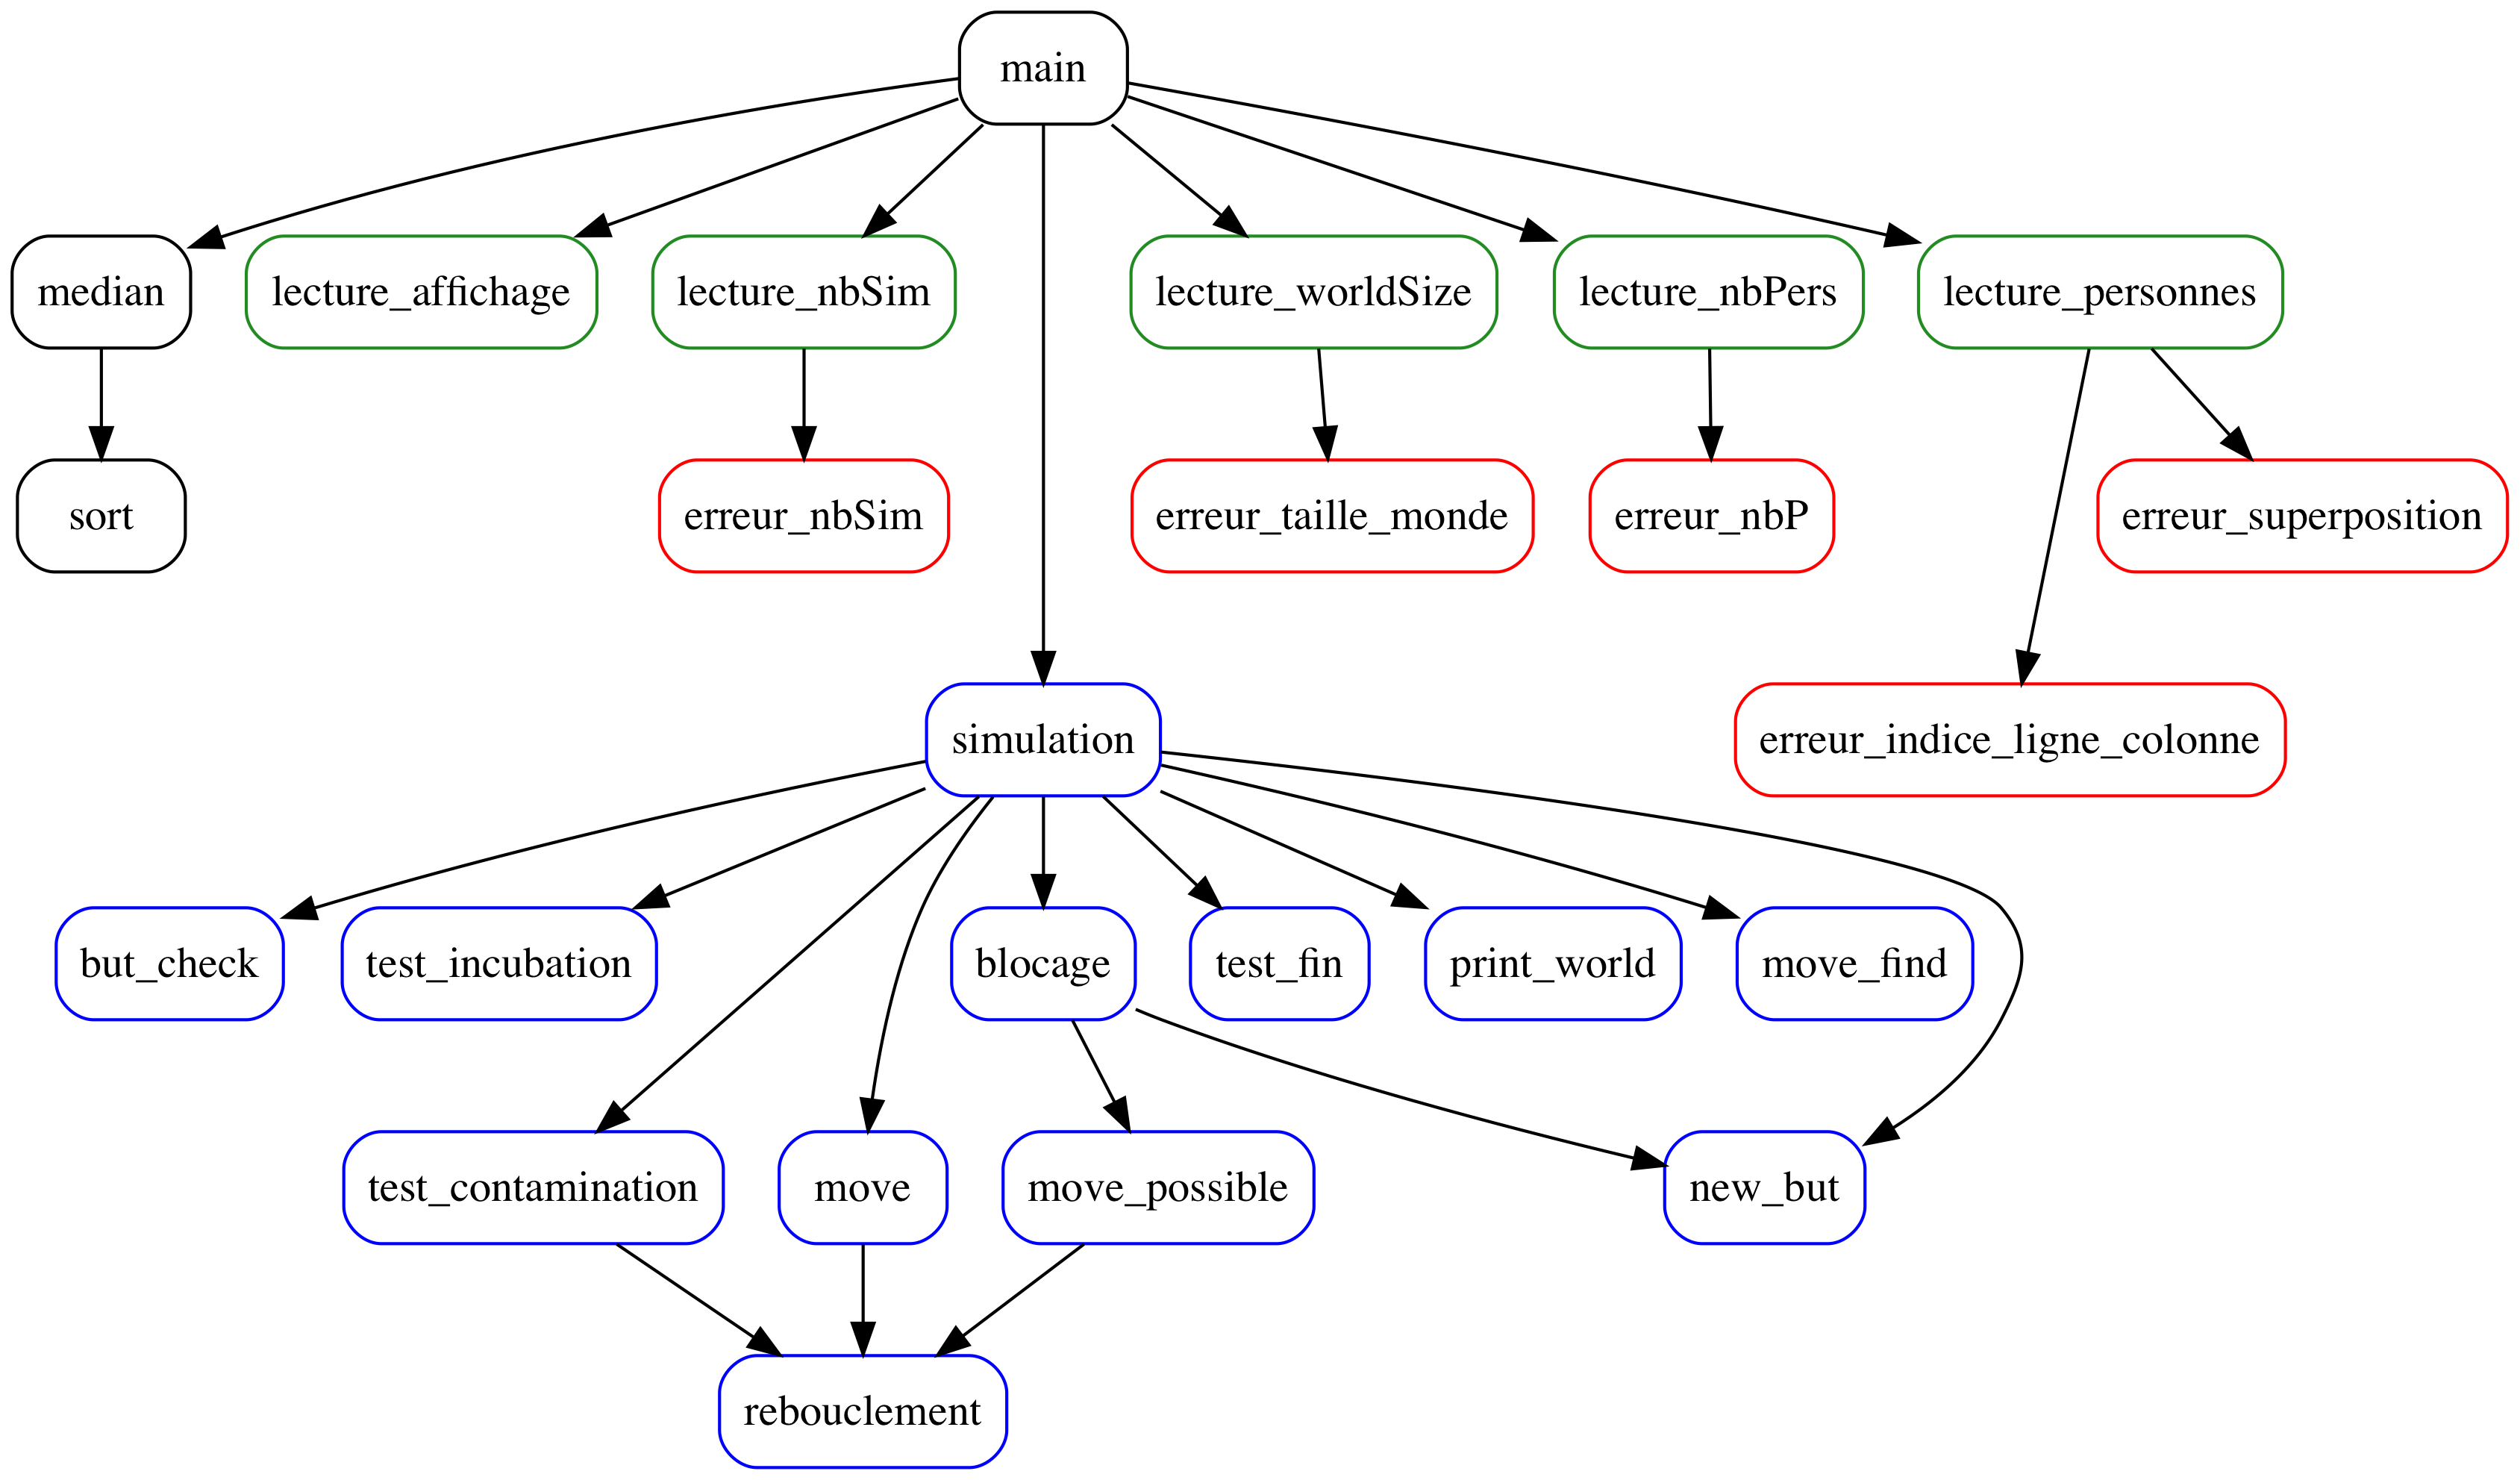
\includegraphics[scale=0.11]{graph.png}
\end{framed}
\caption{Diagramme des fonctions}
\end{figure}
\begin{figure}[htb]
\begin{framed}

\end{framed}
\caption{Pseudocode}
\end{figure}


\end{document}  